\documentclass[DM,authoryear,toc]{lsstdoc}
% lsstdoc documentation: https://lsst-texmf.lsst.io/lsstdoc.html
\input{meta}

% Package imports go here.
\usepackage{listings}
\usepackage{color}

\definecolor{dkgreen}{rgb}{0,0.6,0}
\definecolor{gray}{rgb}{0.5,0.5,0.5}
\definecolor{mauve}{rgb}{0.58,0,0.82}

\newenvironment{allintypewriter}{\ttfamily}{\par}

\lstset{frame=tb,
  language=SQL,
  aboveskip=3mm,
  belowskip=3mm,
  showstringspaces=false,
  columns=flexible,
  basicstyle={\small\ttfamily},
  numbers=none,
  numberstyle=\tiny\color{gray},
  keywordstyle=\color{blue},
  commentstyle=\color{dkgreen},
  stringstyle=\color{mauve},
  breaklines=true,
  breakatwhitespace=true,
  tabsize=3
}


% Local commands go here.

%If you want glossaries
%\input{aglossary.tex}
%\makeglossaries

\title{Validation Tests of the DP0.1 TAPserver on IDF}

% Optional subtitle
% \setDocSubtitle{A subtitle}

\author{%
Douglas L.\ Tucker
}

\setDocRef{RTN-026}
\setDocUpstreamLocation{\url{https://github.com/lsst/rtn-026}}

\date{\vcsDate}

% Optional: name of the document's curator
% \setDocCurator{The Curator of this Document}

\setDocAbstract{%
  DP0.1 contains the ``wide-fast-deep'' (WFD)
  simulated data set from the Vera C. Rubin LSST DESC DR2.  This data
  set contains, among other material, images and catalogs for c.\ 300
  sq deg of contiguous sky within the LSST footprint.  Here, we
  present verfication tests of the catalog data contained within the
  DP0.1 TAPserver on the Interim Data Facility (IDF).  }

% Change history defined here.
% Order: oldest first.
% Fields: VERSION, DATE, DESCRIPTION, OWNER NAME.
% See LPM-51 for version number policy.
\setDocChangeRecord{%
  \addtohist{1}{YYYY-MM-DD}{Unreleased.}{Douglas Tucker}
}


\begin{document}

% Create the title page.
\maketitle
% Frequently for a technote we do not want a title page  uncomment this to remove the title page and changelog.
% use \mkshorttitle to remove the extra pages

% ADD CONTENT HERE
% You can also use the \input command to include several content files.

\section{Introduction} \label{sec:intro}

This Rubin Technical Note (RTN-026) documents the validation of the
TAP service (Qserv) database on the Interim Data Facility (IDF) for
DP0.1.  DP0.1 contains the “wide-fast-deep” (WFD) simulated data set
from the Vera C.\ Rubin LSST Dark Energy Science Collaboration (DESC)
Data Challege 2 (DC2) \citep{2021ApJS..253...31L,
  2021arXiv210104855L}.  This data set contains, among other material,
images and catalogs for c.\ 300 sq deg of contiguous sky within the
LSST footprint.  The processing for DP0.1 was performed by IN2P3 on a
now-deprecated version of the Data Management (DM) Stack.  The raw and
processed DP0.1 data were first transferred from IN2P3 to NCSA in
December 2020 and January 2021, and transferred to the Interim Data
Facility (IDF) on the Google Web Services (GWS) over the next couple
months.  Transfer to the IDF was declared completed on 31 March 2021,
and DP0.1 was released to an initial group of c.\ 225 DP0 Delegates on
30 June 2021.  DP0.2 will cover the same raw data as DP0.1, but will
be processed with a newer version of the DM Stack.  DP0 as a whole
(which includes both DP0.1 and DP0.2) is described in \citeds{RTN-001}.

Here, we present the results of validation tests of the DP0.1 catalog
data contained within the DP0.1 Qserv database on the IDF.  For the
most part, we used the Jupyter notebook interface to the TAP service
on the Rubin Science Platform (RSP) on the IDF to access the Qserv
DP0.1 database, although we occaionally used the National Virtual
Observatory (NVO) TOPCAT java software package for initial tests.

Access via the Jupyter notebook interface was achieved via the
following code:

\begin{lstlisting}[
    language=Python,
    label={lst:access},
    caption={Accessing Qserv via the RSP@IDF JupyterLab environment.},
    captionpos=b]
# Import the Rubin TAP service utilities
from rubin_jupyter_utils.lab.notebook import get_tap_service, retrieve_query, get_catalog
# Get an instance of the TAP service
service = get_tap_service()
assert service is not None
assert service.baseurl == "https://data.lsst.cloud/api/tap"
\end{lstlisting}



\section{Basic Tests of the \texttt{dp01\_dc2\_catalalogs} Schema} \label{sec:basic}

As a first basic test of the DP0.1 contents of Qserv, we looked at which tables were available in the
\texttt{dp01\_dc2\_catalogs} schema:

%\lstset{language=Python}
\begin{lstlisting}[
    language=Python,
    label={lst:tables_query},
    caption={Querying tables in the Qserv \texttt{dp01\_dc2\_catalogs} schema.},
    captionpos=b]
%%time
now0=datetime.now()
schema_name = 'dp01_dc2_catalogs'
query = """SELECT table_name FROM TAP_SCHEMA.tables WHERE schema_name=%s""" % ("\'"+schema_name+"\'")
print(query)
results = service.search(query)
df = results.to_table().to_pandas()
table_full_name_list = df['table_name'].tolist()
print(table_full_name_list)
\end{lstlisting}

Here are the results, which match expectations:

%\lstset{language=Python}
\begin{lstlisting}[
    language=Python,
    label={lst:tables_result},
    caption={Results from query in Listing~\ref{lst:tables_query}.},
    captionpos=b]
SELECT table_name FROM TAP_SCHEMA.tables WHERE schema_name='dp01_dc2_catalogs'
['dp01_dc2_catalogs.forced_photometry', 'dp01_dc2_catalogs.object', 'dp01_dc2_catalogs.position', 'dp01_dc2_catalogs.reference', 'dp01_dc2_catalogs.truth_match']
CPU times: user 17 ms, sys: 0 ns, total: 17 ms
yWall time: 60.7 ms
\end{lstlisting}


Once we we checked that the above tables were, in fact, in the IDF Qserv database, our next simple test was to check how many records (rows) there were in these 5 tables: 

%\lstset{language=Python}
\begin{lstlisting}[
    language=Python,
    label={lst:tables_numrecords_query},
    caption={Querying total number of records in each table in the \texttt{dp01\_dc2\_catalogs} schema.},
    captionpos=b]
for table in ['forced_photometry', 'object', 'position', 'reference', 'truth_match']:
   query = """SELECT count(*) FROM dp01_dc2_catalogs.%s""" % (table)
   print(query)
   results = service.search(query)
   df = results.to_table().to_pandas()
   count = df['count'].iloc[0]
   print(count)
   print("")
\end{lstlisting}

Here are the results:

%\lstset{language=SQL}
\begin{lstlisting}[
    language=Python,
    label={lst:tables_numrecords_results},
    caption={Results from query in Listing~\ref{lst:tables_numrecords_query}.},
    captionpos=b]
SELECT count(*) FROM dp01_dc2_catalogs.forced_photometry
147088445

SELECT count(*) FROM dp01_dc2_catalogs.object
147088478

SELECT count(*) FROM dp01_dc2_catalogs.position
147088445
 
SELECT count(*) FROM dp01_dc2_catalogs.reference
147088445

SELECT count(*) FROM dp01_dc2_catalogs.truth_match
765823615
\end{lstlisting}

As expected, the \texttt{forced\_photometry}, \texttt{object},
\texttt{position}, and \texttt{reference} tables have a (nearly)
identical number of rows, since each of these tables refers to
individual objects that are the same for all four of these tables.
(It has been noted that the \texttt{object} table contains 33 more
rows than the other three of these four tables, but why this is so has
yet to be fully investigated.)  The \texttt{truth\_match} has
$\approx$5$\times$ as many entries as the other four catalogs.  A
quick check indicates that \texttt{truth\_match} contains a
considerable number of objects with no match in (say) the
\texttt{object} table, and the peak of \texttt{r\_mag} for entries in
the \texttt{truth\_match} is $\approx$29.0 instead of $\approx$26.0 as it is
for the \texttt{object} table (see
Fig.~\ref{fig:truth_match_object_mag_r}); so we can surmise that, overall,
the \texttt{truth\_match} table is much deeper.  If we constrain the above
query on \texttt{truth\_match} to only those entries for which
\texttt{truth\_match.match\_objectId}$>-1$, we find 147088478 entries,
the same as in the \texttt{object} table.

\begin{figure*}
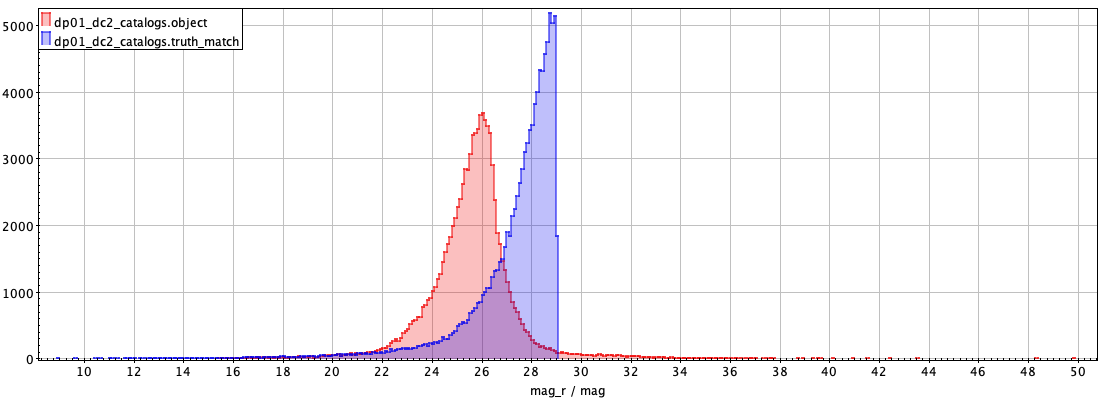
\includegraphics[width=1.0\textwidth]{Plots/truth_match_object_mag_r.png}
\caption{The distribution of $r$-band magnitudes for the first 100,000 rows returned from \texttt{dp01\_dc2\_catalogs.object} and from \texttt{dp01\_dc2\_catalogs.truth\_match}.  Note that the distribution of $r$-band magnitudes for \texttt{dp01\_dc2\_catalogs.truth\_match} is skewed much fainter than that for \texttt{dp01\_dc2\_catalogs.object}.  \texttt{dp01\_dc2\_catalogs.truth\_match}  clearly holds a superset of objects of which only $\approx20\%$ are included in the \texttt{dp01\_dc2\_catalogs.object} (and other) tables.
 }
\label{fig:truth_match_object_mag_r}
\end{figure*}



\section{More Detailed Tests of Individual Tables in the  \texttt{dp01\_dc2\_catalalogs} Schema} \label{sec:detailed}

A separate Jupyter notebook was created to test in more detail the
contents of each table in the \texttt{dp01\_dc2\_catalalogs} schema.
In each case, similar steps were followed:
\begin{enumerate}
\item Import a set of standard python modules (\texttt{numpy},
  \texttt{pandas}, etc.) as well the RSP@IDF TAP service utilities.
\item Obtain an instance of the TAP service at
  \url{https://data.lsst.cloud/api/tap}.
\item Verify the counts of entries for the table as was done in the
  general schema tests (Section~\ref{sec:basic}).
\item Verify the list of tracts as also was done in the general schema
  tests (Section~\ref{sec:basic}).
\item Loop over each tract:
  \begin{enumerate}
  \item Query for the full contents of the table for that tract (via
    asynchronous TAP query).
  \item Load the results of the query in a Pandas data frame.
  \item For each column in the Pandas data frame:
    \begin{enumerate}
    \item Count the total number of entries and the number of entries
      with a value of \texttt{NaN}.
    \item Calculate the 1-percentile, the 50-percentile (median), and the
      99-percentile value for that column via the Pandas
      \texttt{Series.quantile} function.
    \end{enumerate}
  \end{enumerate}
\item Once the the above statistics are measured for each column in
  each tract, compile the histogram showing the distribution of these
  statistics over all 166 tracts for each column.
\item Once all the above is completed for a given table, the
  asynchronous TAP jobs can be deleted.
\end{enumerate}

Details of this process can be viewed in the rendered Jupyter notebooks at
\url{https://github.com/lsst/rtn-026/blob/master/notebooks/}.


Note, the process of querying a table for all its entries
tract-by-tract and downloading to a Pandas data frame is very
resource- and time-intensive.  Typically, the process to analyze a
single table would take $\gtrsim$16 hours of wall clock time.  In
fact, this was not possible for one of the tables
(\texttt{forced\_photometry}), and a different, more approximate
method needed to be employed.

We note that `tract` is only included as a column in the
\texttt{object} and in the \texttt{truth\_match} tables; for the other
tables, we perform an inner join with the \texttt{object} table on the
`objectId` column, which is a column in all five tables.  Here is the
basic code for compiling the list of tracts for those tables that do
not include a `tract` column (Step 4 in the above list of steps for the
detailed tests of the individual tables):
%\lstset{language=Python}
\begin{lstlisting}[
    language=Python,
    label={lst:tracts_query},
    caption={Querying distinct \texttt{tracts} available in DP0.1.},
    captionpos=b]
%%time
now0=datetime.now()
# `tract` is not a column in several of the tables; so we need to be a little tricky...
query = """SELECT DISTINCT obj.tract 
           FROM %s.object as obj
           JOIN %s as x
           ON obj.objectId = x.objectId  
           ORDER BY obj.tract""" % \
        (schema_name, table_full_name)
print(query)
results = service.search(query)
df = results.to_table().to_pandas()
tract_list = df['tract'].tolist()
now1=datetime.now()
print("Total time:", now1-now0)
print(tract_list)
\end{lstlisting}

And here are the results, using the \texttt{position} table as an example:
%\begin{allintypewriter}
%\lstset{language=sh}
\begin{lstlisting}[
    language=Python,
    label={lst:tracts_results},
    caption={Results of query in Listing~\ref{lst:tracts_query} for one of the tables.},
    captionpos=b]
SELECT DISTINCT obj.tract 
           FROM dp01_dc2_catalogs.object as obj
           JOIN dp01_dc2_catalogs.position as x
           ON obj.objectId = x.objectId  
           ORDER BY obj.tract
Total time: 0:01:53.352097
[2723, 2724, 2725, 2726, 2727, 2728, 2729, 2730, 2731, 2732, 2733, 2734, 2735, 2896, 2897, 2898, 2899, 2900, 2901, 2902, 2903, 2904, 2905, 2906, 2907, 2908, 3074, 3075, 3076, 3077, 3078, 3079, 3080, 3081, 3082, 3083, 3084, 3085, 3086, 3256, 3257, 3258, 3259, 3260, 3261, 3262, 3263, 3264, 3265, 3266, 3267, 3268, 3441, 3442, 3443, 3444, 3445, 3446, 3447, 3448, 3449, 3450, 3451, 3452, 3453, 3454, 3631, 3632, 3633, 3634, 3635, 3636, 3637, 3638, 3639, 3640, 3641, 3642, 3643, 3825, 3826, 3827, 3828, 3829, 3830, 3831, 3832, 3833, 3834, 3835, 3836, 3837, 4022, 4023, 4024, 4025, 4026, 4027, 4028, 4029, 4030, 4031, 4032, 4033, 4034, 4035, 4224, 4225, 4226, 4227, 4228, 4229, 4230, 4231, 4232, 4233, 4234, 4235, 4236, 4429, 4430, 4431, 4432, 4433, 4434, 4435, 4436, 4437, 4438, 4439, 4440, 4441, 4636, 4637, 4638, 4639, 4640, 4641, 4642, 4643, 4644, 4645, 4646, 4647, 4648, 4850, 4851, 4852, 4853, 4854, 4855, 4856, 4857, 4858, 4859, 4860, 5065, 5066, 5067, 5068, 5069, 5070, 5071, 5072, 5073, 5074]
CPU times: user 12.5 ms, sys: 3.93 ms, total: 16.4 ms
Wall time: 1min 53s
\end{lstlisting}
%\end{allintypewriter}



\subsection{\texttt{object} Table} \label{sec:object}

We provide in the Appendix code listings for the most important parts
of Jupyter notebook written for the detailed analysis of the \texttt{object table}.
As noted previously, the rendered notebooks for the general and the detailed analyses of
all the tables can be found here:
\url{https://github.com/lsst/rtn-026/blob/master/notebooks/}.

In the Appendix, Listing~\ref{lst:object_urls} shows how asynchronous
TAP queries are performed on a `tract` by `tract` basis and saved for
later analysis.  The queries are done asynchronously and the URLs to
the results are saved since this step takes several hours.  Saving the
results allows us to start up again from where the job crashed if the
connection happens to fail.

Listing~\ref{lst:object_tracts} shows how the statistics are derived
for each of the 166 `tracts`.  In the previous step (Step 5(a);
Listing~\ref{lst:object_urls}), the whole contents of each `tract` is
downloaded and saved at a URL.  In this step (Step 5(b)\&(c)), the URL
for each `tract` is read into a Pandas `DataFrame` and a set of
statistics is calculated for that `tract` for each column of the 
\texttt{object} table:
\begin{itemize}
\item the total number of rows in that column for that `tract`, $N_{\rm tot}$;
\item the total number of rows in that column for that `tract` which have NaN as the value, $N_{\rm NaN}$;
\item the fraction of rows in that column for that `tract` with NaN as the value ($N_{\rm NaN} / N_{\rm tot}$);
\item the 1-percentile value of that column for that `tract`;
\item the 50-percentile (median) value of that column for that `tract`; and 
\item the 99-percential value of that column for that `tract`.
\end{itemize}

Listing~\ref{lst:object_plots} shows how the statistics for each
column for each `tract` described in the previous step (Step
5(b)\&(c); Listing~\ref{lst:object_tracts}) are compiled and their
distributions are plotted.  For each column from the original table, a
figure containing 6 sub-plots -- a histogram for each of the above 6
statistics -- is created.

After Step 6 (Listing~\ref{lst:object_plots}), the results from the
asynchronous TAP jobs can be deleted.

For the \texttt{object} table, over 100 plots -- each with 6 sub-plots
-- are created, one plot for each ``plottable'' column.  Here, we show
3 representative plots: one for the `mag\_i` column
(Fig.~\ref{fig:object_mag_i}), one for the `magerr\_i` column
(Fig.~\ref{fig:object_magerr_i}), and one for the `psf\_fwhm\_i` column
(Fig.~\ref{fig:object_psf_fwhm_i}).

A gzip-compressed tar file containing all 100$+$ plots for the
\texttt{object} table can be found here:
\url{https://github.com/lsst/rtn-026/tree/master/Plots}.

\begin{figure*}[h]
\centering
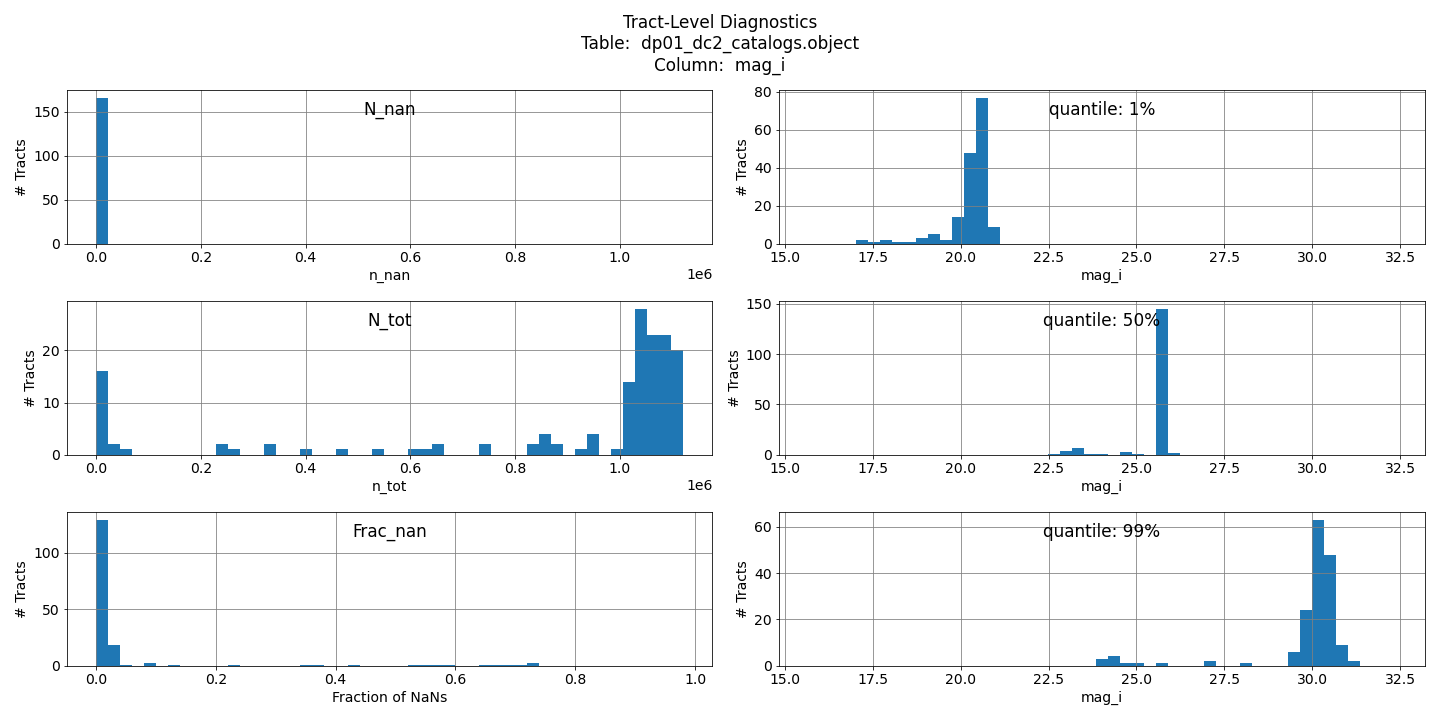
\includegraphics[width=1.0\linewidth]{Plots/TAP_verify_DP01.dp01_dc2_catalogs.object.mag_i.png}
\caption{}
\label{fig:object_mag_i}
\end{figure*}

\begin{figure*}[h]
\centering
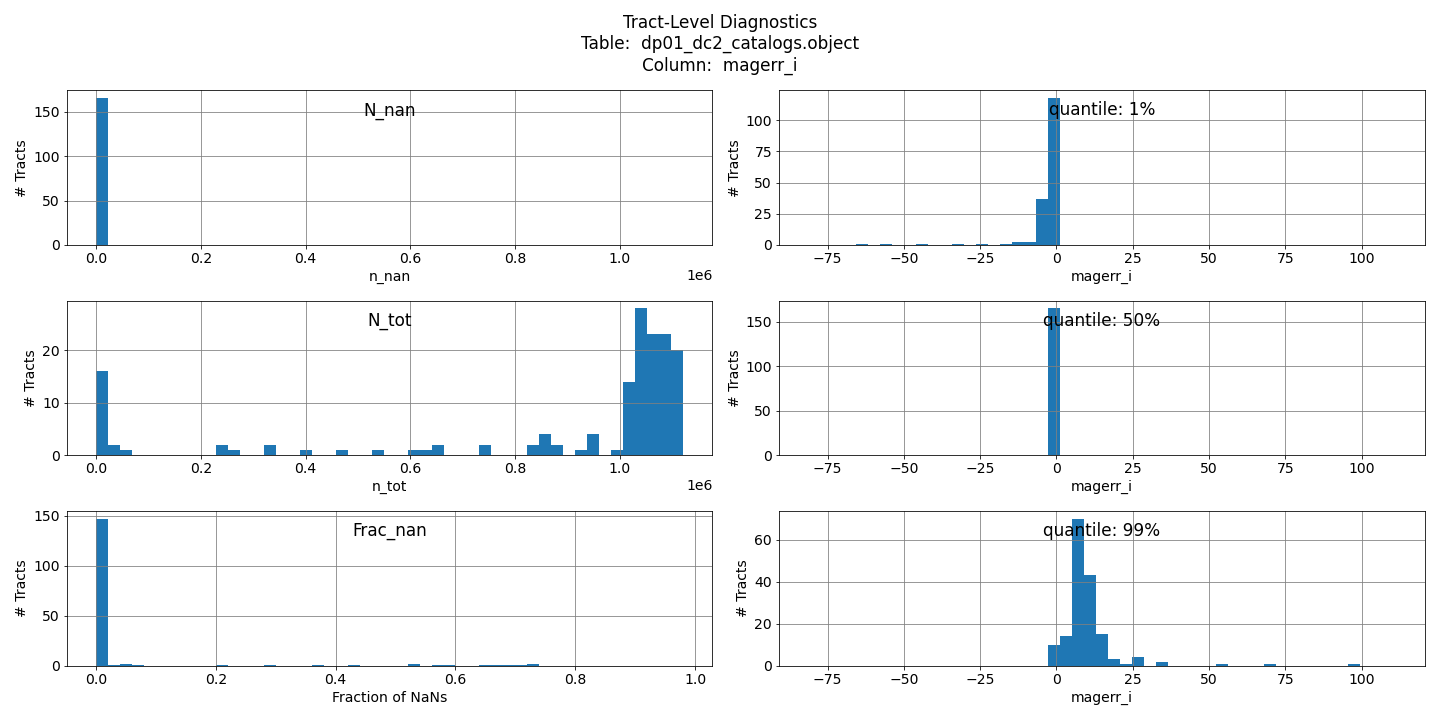
\includegraphics[width=1.0\linewidth]{Plots/TAP_verify_DP01.dp01_dc2_catalogs.object.magerr_i.png}
\caption{}
\label{fig:object_magerr_i}
\end{figure*}

\begin{figure*}[h]
\centering
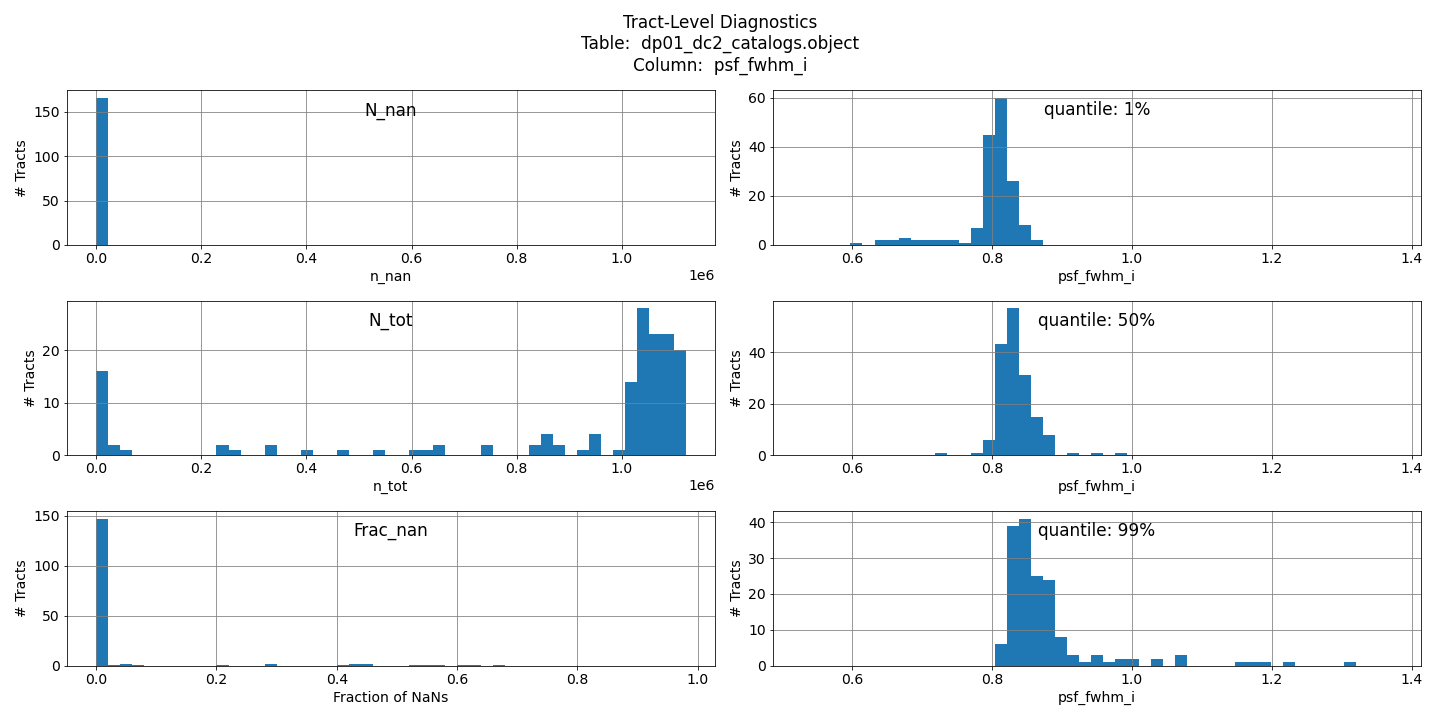
\includegraphics[width=1.0\linewidth]{Plots/TAP_verify_DP01.dp01_dc2_catalogs.object.psf_fwhm_i.png}
\caption{}
\label{fig:object_psf_fwhm_i}
\end{figure*}

We feel that these plots all look ``not unreasonable''.  We hope to
perform more drill-down for DP0.2 and beyond.


%TAP_verify_DP01.dp01_dc2_catalogs.object.mag_i.png
%TAP_verify_DP01.dp01_dc2_catalogs.object.magerr_i.png
%TAP_verify_DP01.dp01_dc2_catalogs.object.psf_fwhm_i.png


\subsection{\texttt{position} Table} \label{sec:position}

The implementation of Steps 5, 6, and 7 from the outline above are
very similar for the \texttt{object} table and for the
\texttt{position} table; so we will not go into the same
level of detail as in Section~\ref{sec:object}.  The \texttt{position}
table, however, has only 4 plottable columns; so we include them all here
(Figs.~\ref{fig:position_coord_ra}--\ref{fig:position_parent}).

A gzip-compressed tar file containing these 4 plots can be found here:
\url{https://github.com/lsst/rtn-026/tree/master/Plots}.

\begin{figure*}[h]
\centering
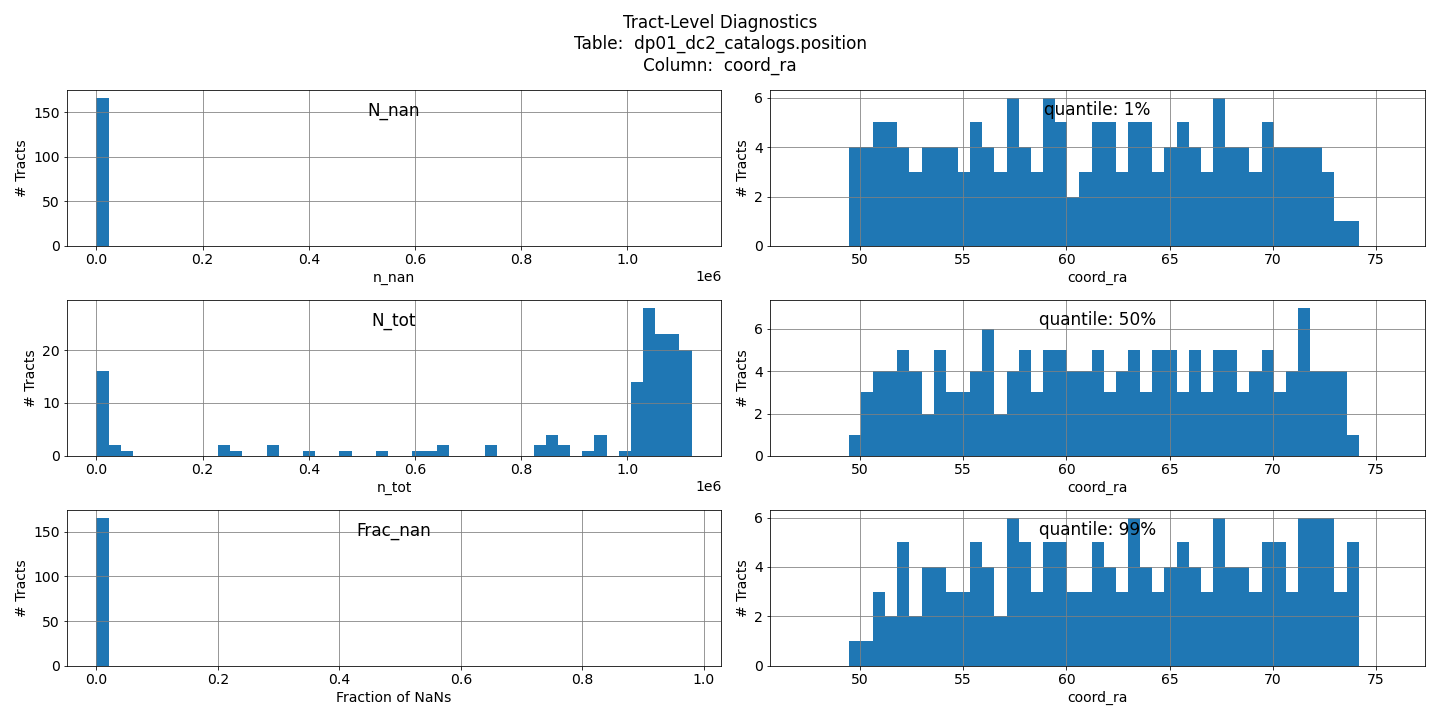
\includegraphics[width=1.0\linewidth]{Plots/TAP_verify_DP01.dp01_dc2_catalogs.position.coord_ra.png}
\caption{}
\label{fig:position_coord_ra}
\end{figure*}

\begin{figure*}[h]
\centering
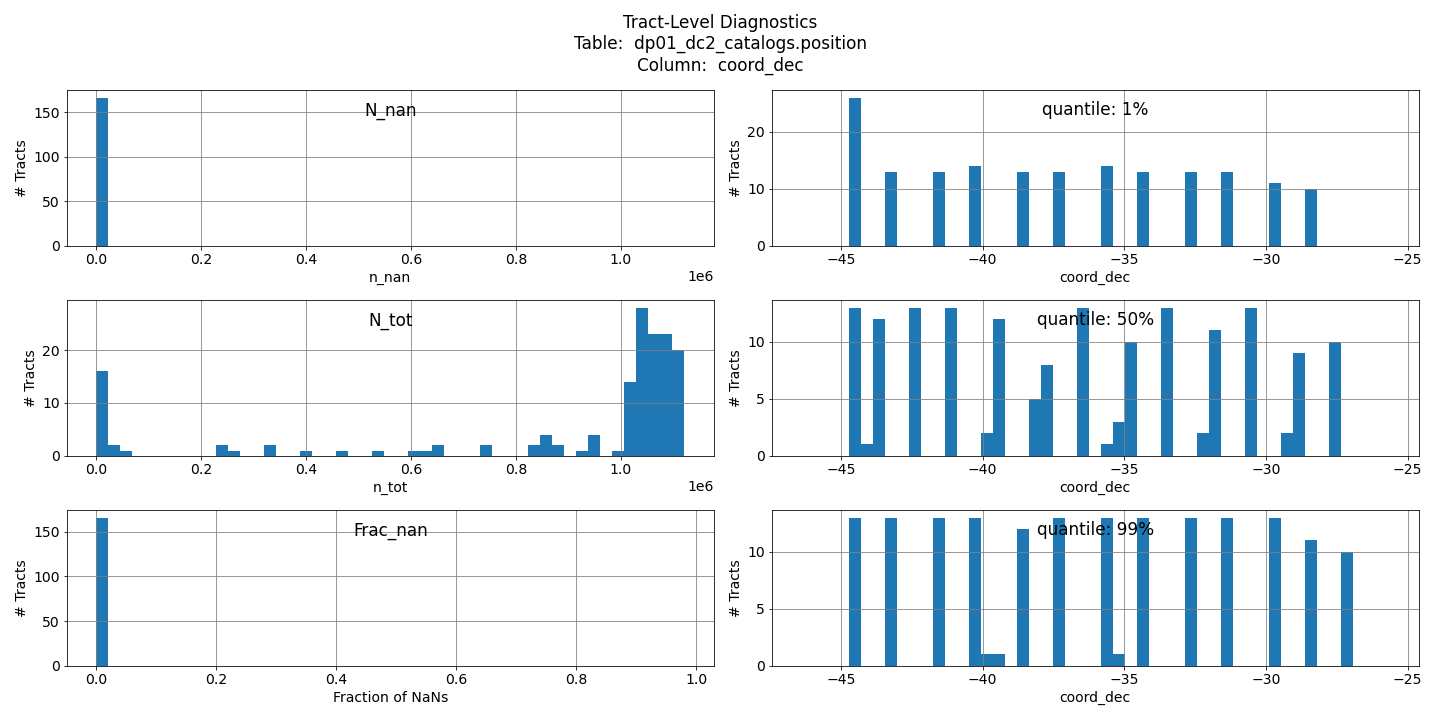
\includegraphics[width=1.0\linewidth]{Plots/TAP_verify_DP01.dp01_dc2_catalogs.position.coord_dec.png}
\caption{}
\label{fig:position_coord_dec}
\end{figure*}

\begin{figure*}[h]
\centering
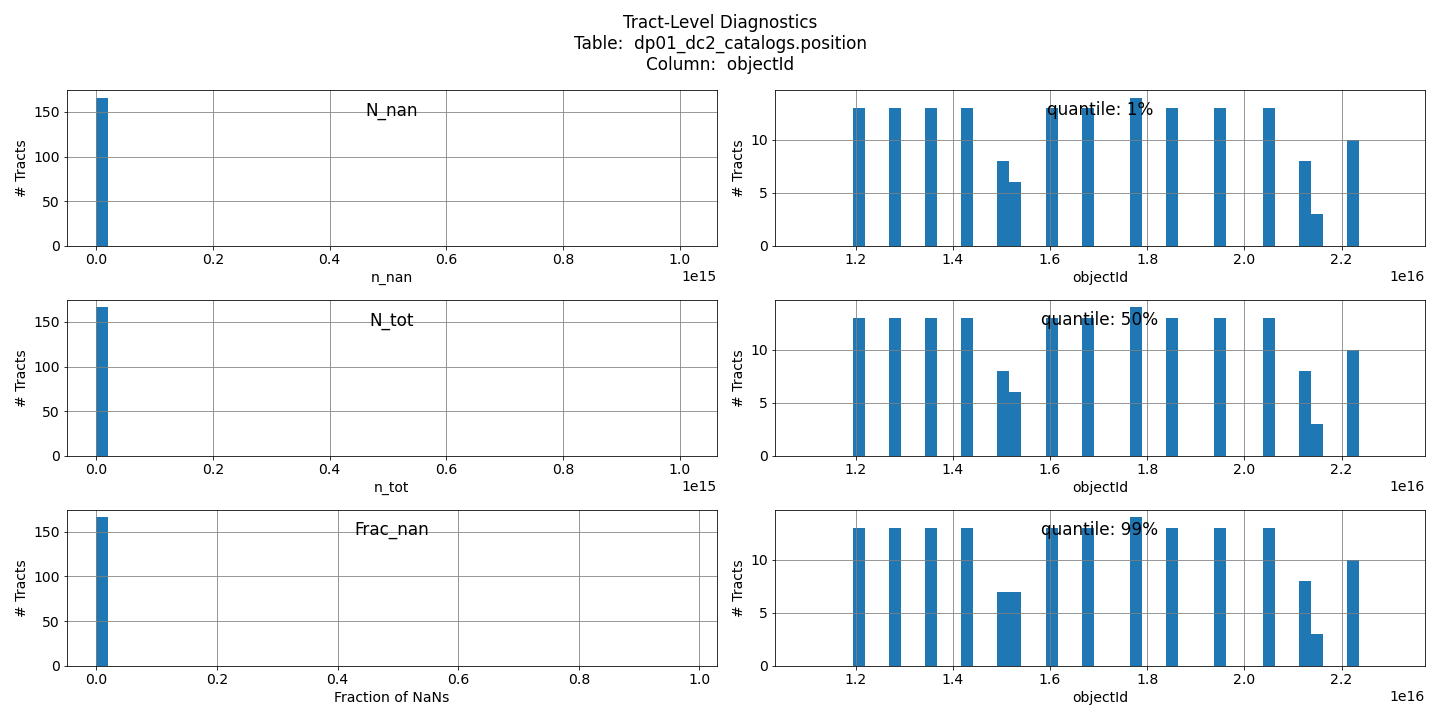
\includegraphics[width=1.0\linewidth]{Plots/TAP_verify_DP01.dp01_dc2_catalogs.position.objectId.png}
\caption{}
\label{fig:position_objectId}
\end{figure*}

\begin{figure*}[h]
\centering
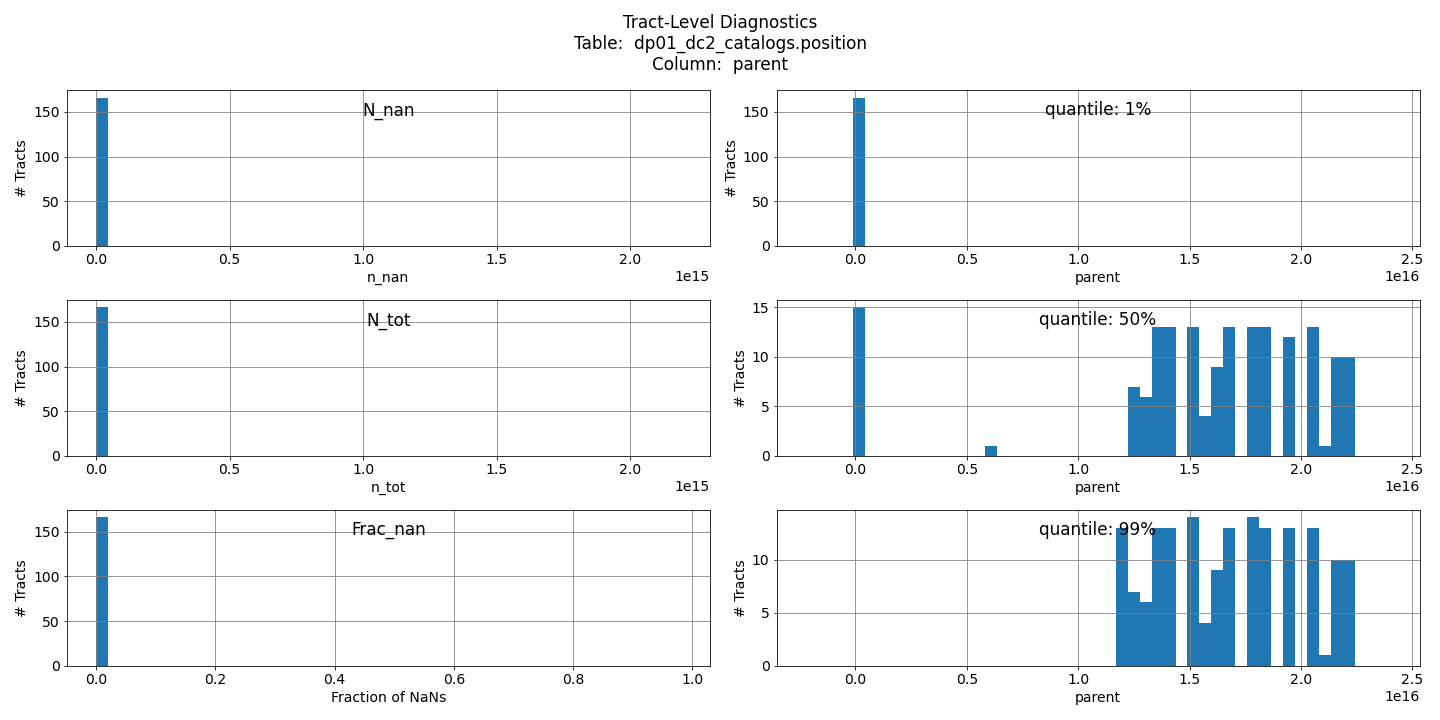
\includegraphics[width=1.0\linewidth]{Plots/TAP_verify_DP01.dp01_dc2_catalogs.position.parent.png}
\caption{}
\label{fig:position_parent}
\end{figure*}


As with the \texttt{object} table plots, we feel that these plots all
look ``not unreasonable'', and we hope to perform more drill-down for
DP0.2 and beyond.





\subsection{\texttt{reference} Table} \label{sec:reference}

As with the \texttt{position} table, the implementation of Steps 5, 6,
and 7 from the outline above are very similar for the \texttt{object}
table and for the \texttt{reference} table; so we will not go into the
same level of detail as in Section~\ref{sec:object}.  The
\texttt{reference} table has over 130 plottable columns; so we
include only 3 representative plots
(Figs.~\ref{fig:reference_base_blendednes_abs}--\ref{fig:reference_deblend_psfcenter_x}).

A gzip-compressed tar file containing all 130$+$ plots table can be
found here: \url{https://github.com/lsst/rtn-026/tree/master/Plots}.


\begin{figure*}[h]
\centering
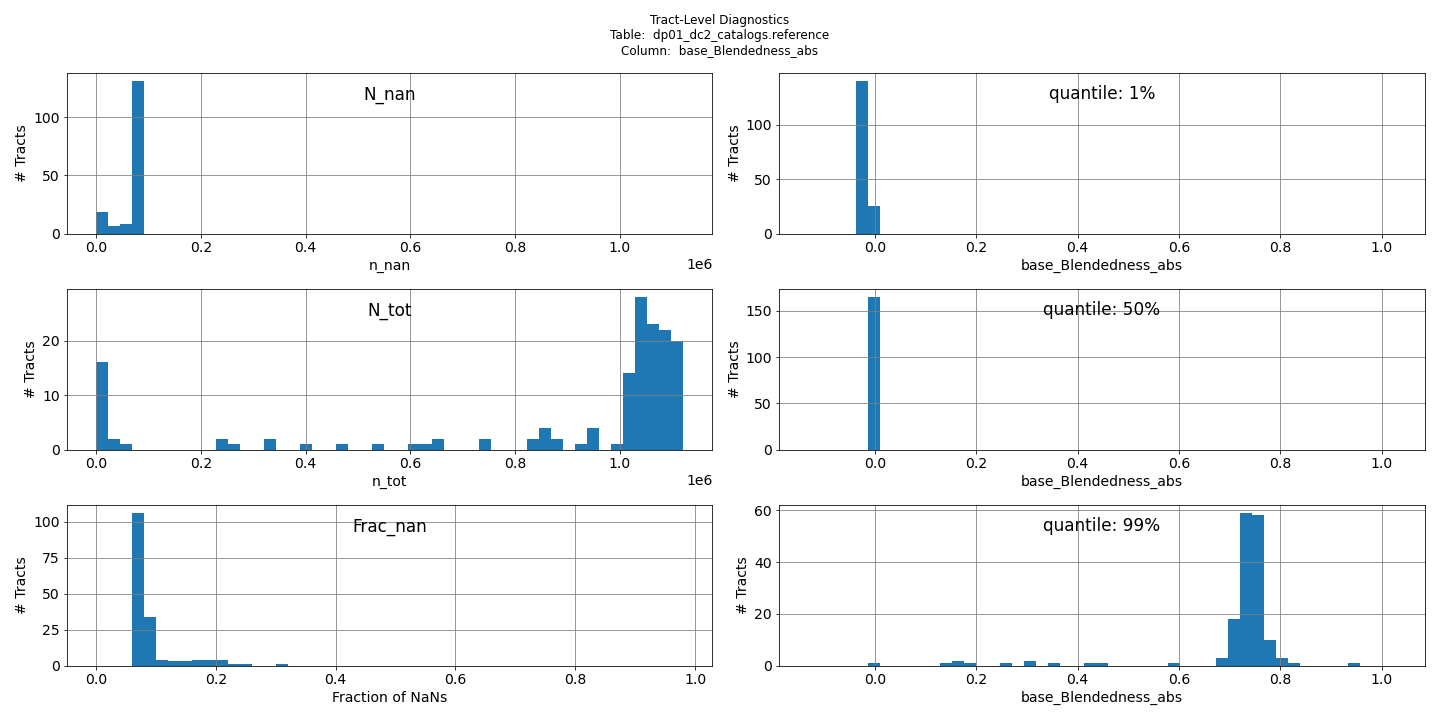
\includegraphics[width=1.0\linewidth]{Plots/TAP_verify_DP01.dp01_dc2_catalogs.reference.base_Blendedness_abs.png}
\caption{}
\label{fig:reference_base_blendednes_abs}
\end{figure*}

\begin{figure*}[h]
\centering
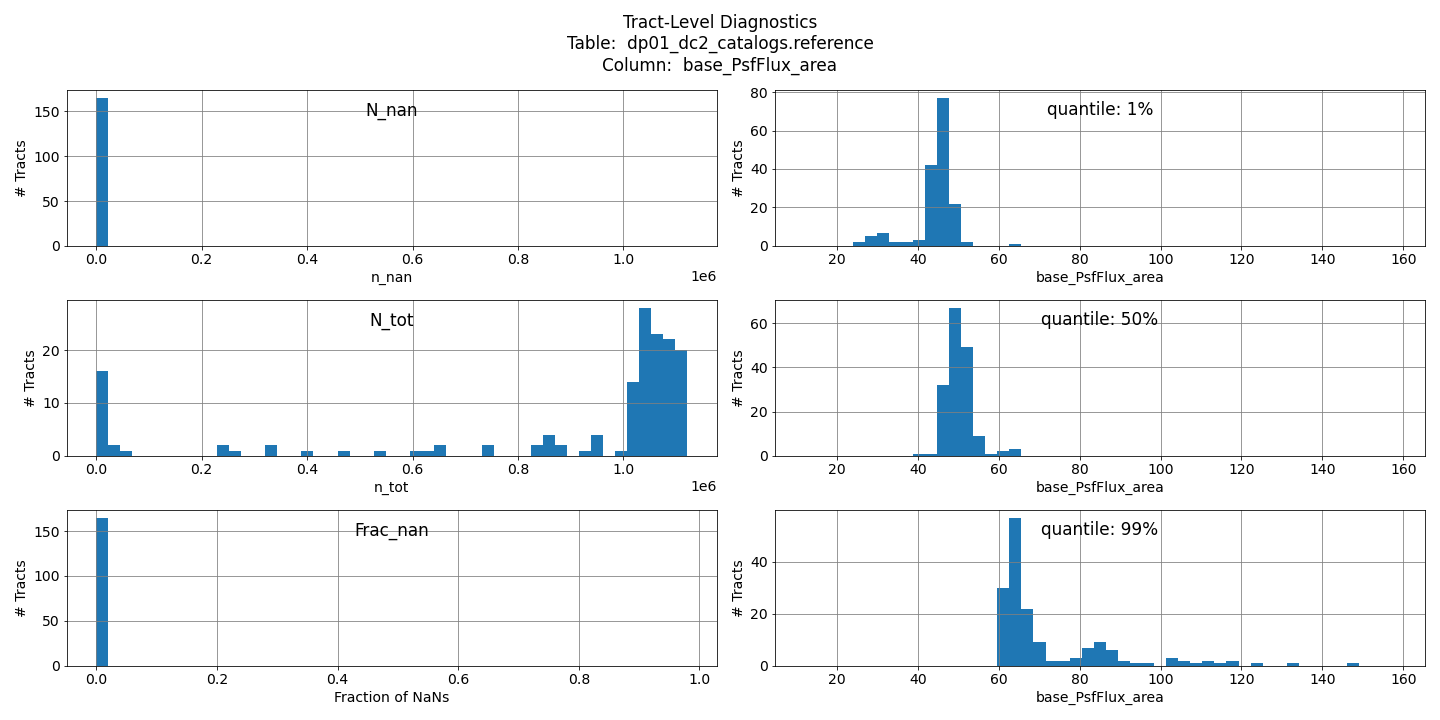
\includegraphics[width=1.0\linewidth]{Plots/TAP_verify_DP01.dp01_dc2_catalogs.reference.base_PsfFlux_area.png}
\caption{}
\label{fig:reference_base_psfflux_area}
\end{figure*}

\begin{figure*}[h]
\centering
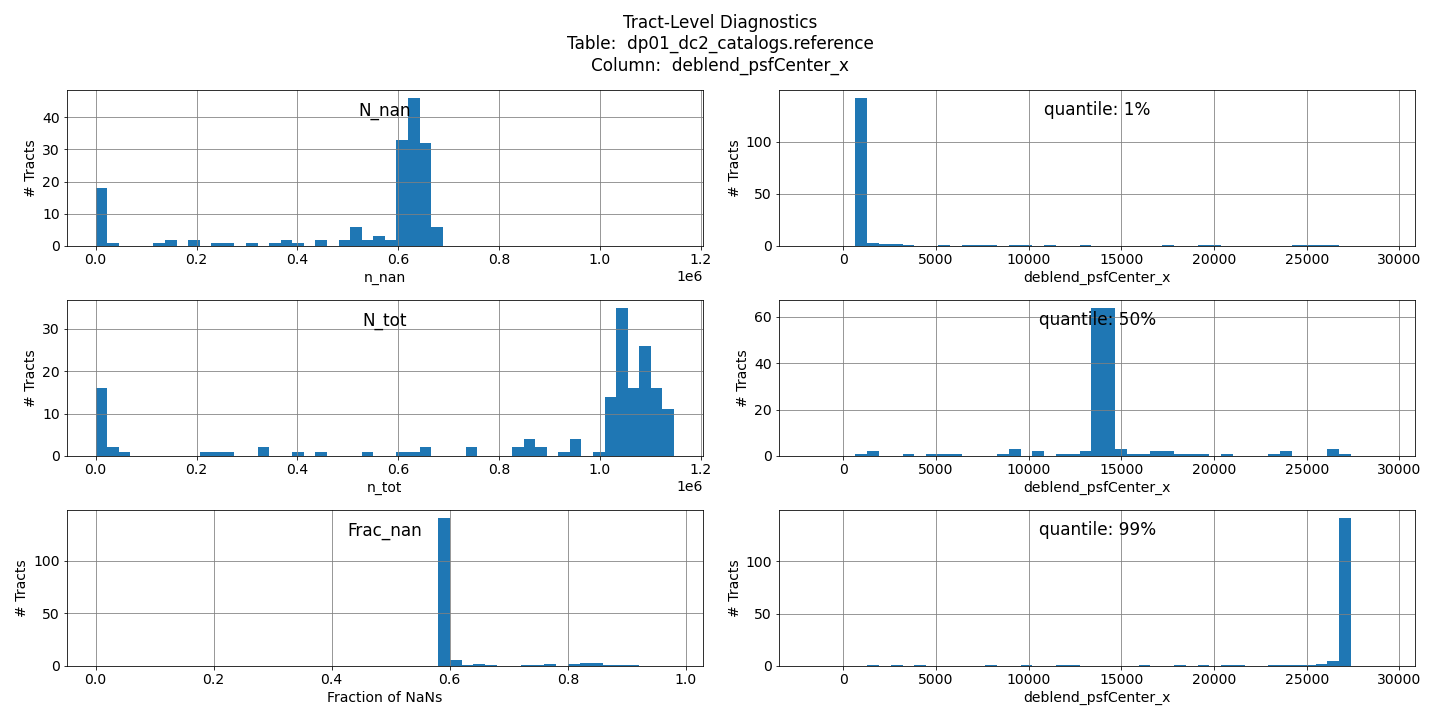
\includegraphics[width=1.0\linewidth]{Plots/TAP_verify_DP01.dp01_dc2_catalogs.reference.deblend_psfCenter_x.png}
\caption{}
\label{fig:reference_deblend_psfcenter_x}
\end{figure*}

As with the histograms plots for the previous tables, we feel that
these plots all look ``not unreasonable'', and we hope to perform more
drill-down for DP0.2 and beyond.


\subsection{\texttt{truth\_match} Table} \label{sec:truth_match}

As with the \texttt{position} and \texttt{reference} tables, the
implementation of Steps 5, 6, and 7 from the outline above are very
similar for the \texttt{object} table and for the \texttt{truth\_match}
table; so we will not go into the same level of detail as in
Section~\ref{sec:object}.  The \texttt{truth\_match} table has 24
plottable columns; so we include only 3 representative plots
(Figs.~\ref{fig:truth_match_flux_i}--\ref{fig:truth_match_redshift}).

A gzip-compressed tar file containing all 24 plots can be found
here: \url{https://github.com/lsst/rtn-026/tree/master/Plots}.



\begin{figure*}[h]
\centering
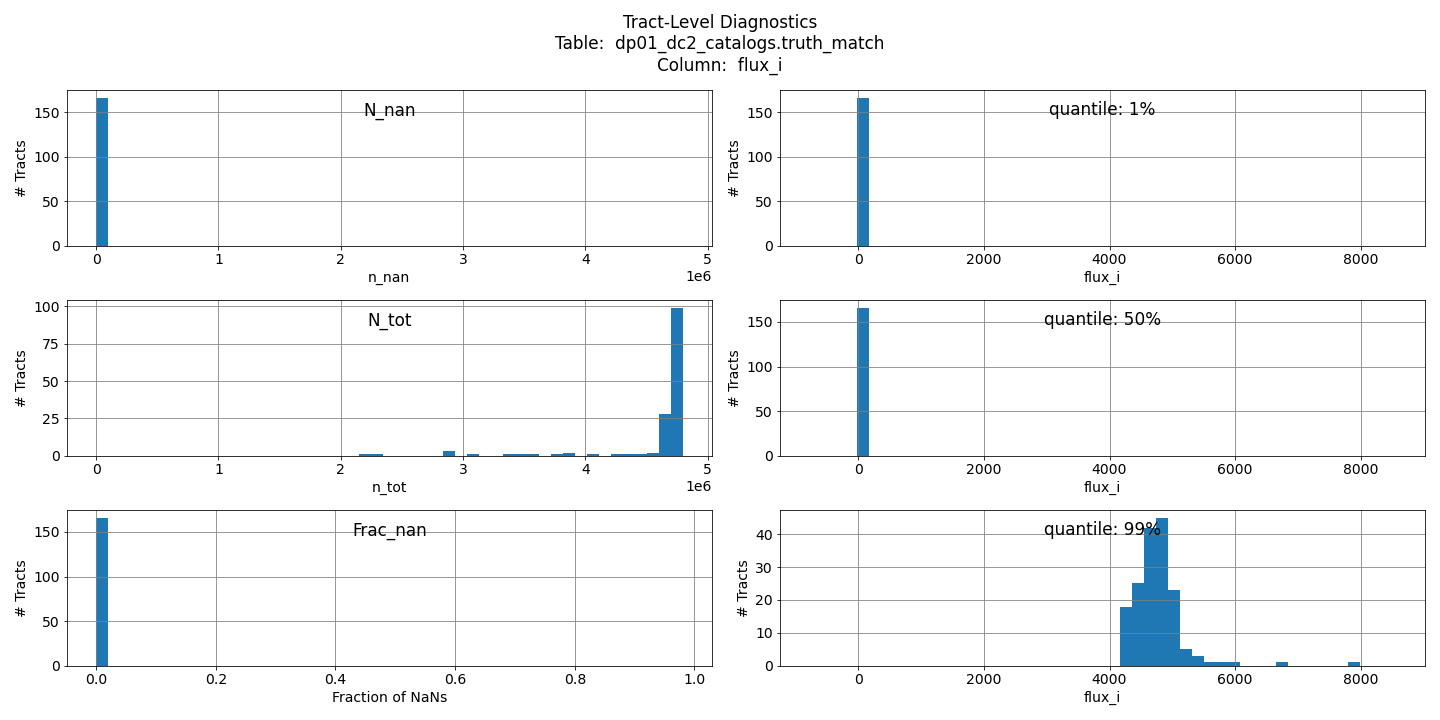
\includegraphics[width=1.0\linewidth]{Plots/TAP_verify_DP01.dp01_dc2_catalogs.truth_match.flux_i.png}
\caption{}
\label{fig:truth_match_flux_i}
\end{figure*}

\begin{figure*}[h]
\centering
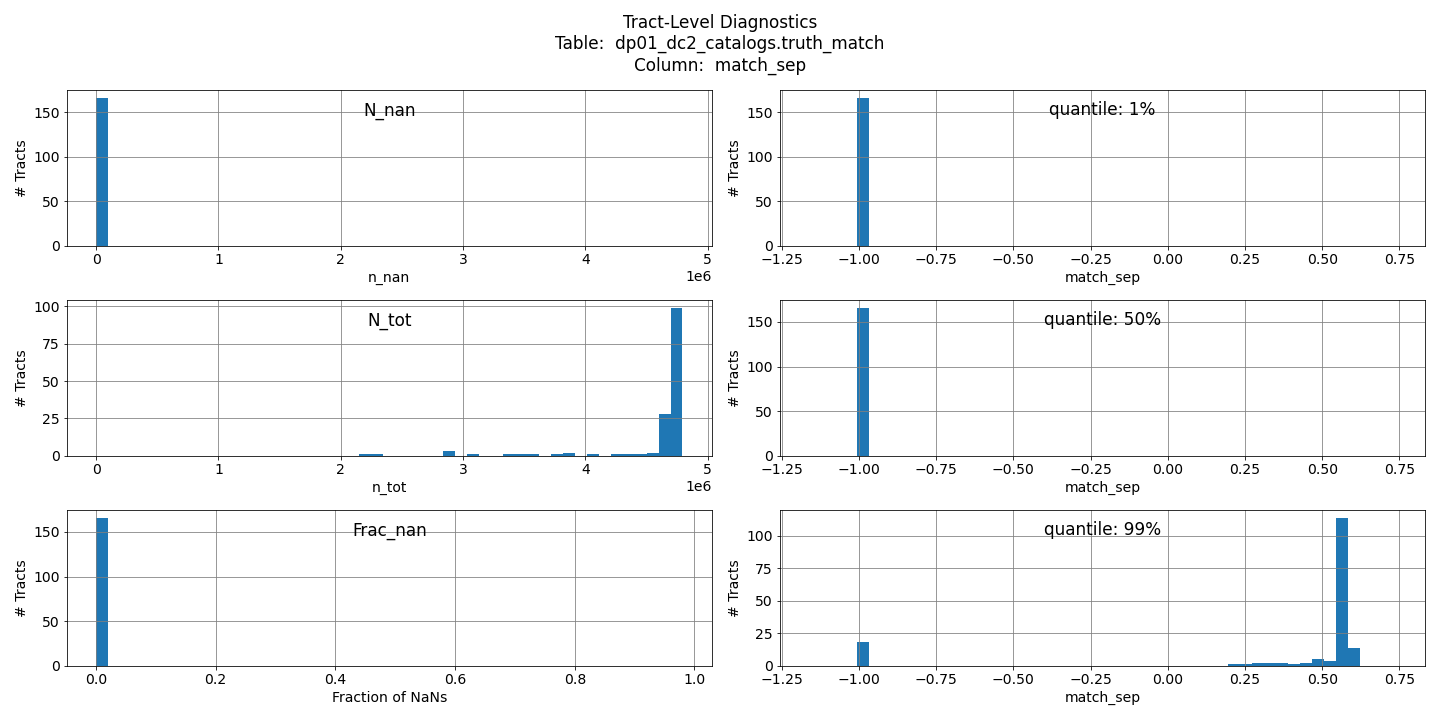
\includegraphics[width=1.0\linewidth]{Plots/TAP_verify_DP01.dp01_dc2_catalogs.truth_match.match_sep.png}
\caption{}
\label{fig:truth_match_match_sep}
\end{figure*}

\begin{figure*}[h]
\centering
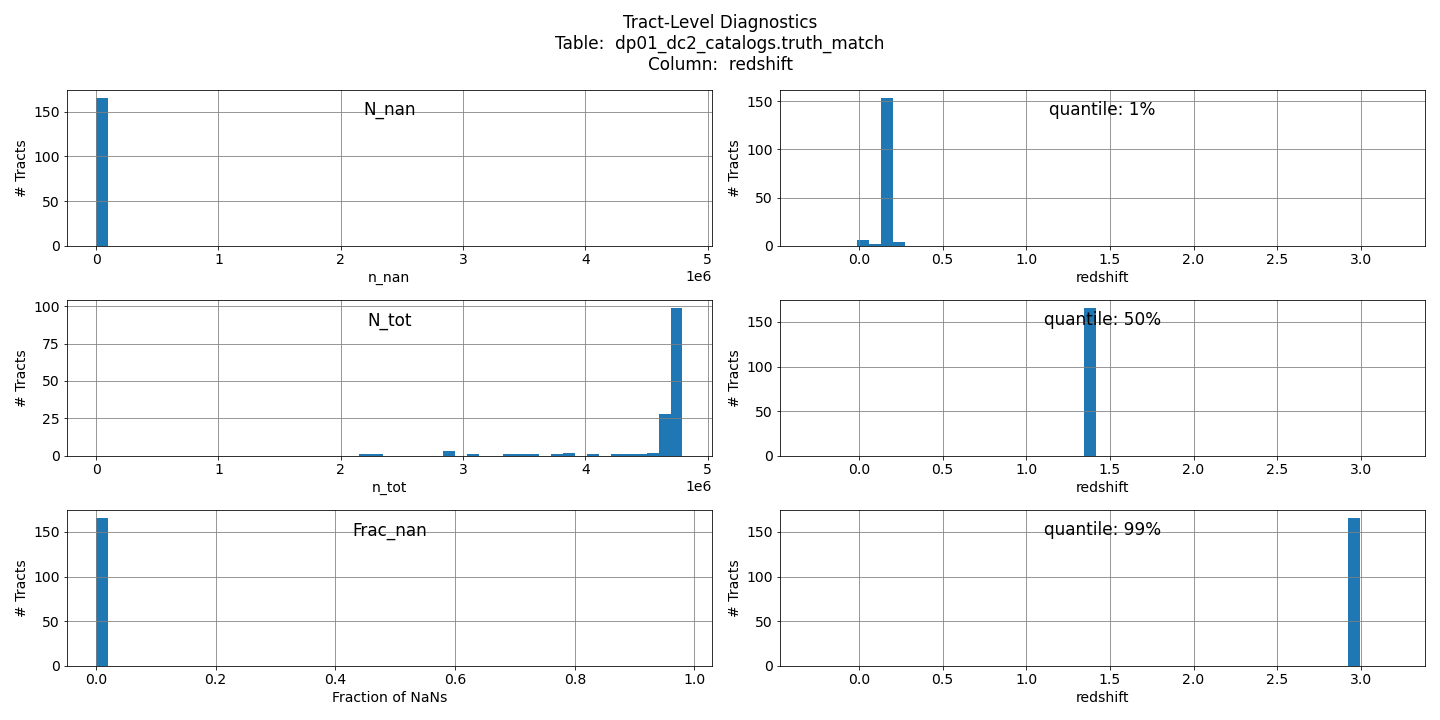
\includegraphics[width=1.0\linewidth]{Plots/TAP_verify_DP01.dp01_dc2_catalogs.truth_match.redshift.png}
\caption{}
\label{fig:truth_match_redshift}
\end{figure*}


As with the histograms plots for the previous tables, we feel that
these plots all look ``not unreasonable'', and we hope to perform more
drill-down for DP0.2 and beyond.


\subsection{\texttt{forced\_photometry} Table} \label{sec:forced_photometry}


\textcolor{red}{\bf{This Section Under Construction.}}


\section{Conclusions} \label{sec:conclusions}

In this Technical Note we have documented basic validation tests of
the IDF DP0.1 Qserv schema and its contents via the RSP TAP service.
These tests included counting the number of records (rows) in each of
the 5 main tables, and then looking in more detail at the contents of
each column of each of the 5 main tables.  This detailed look included
gathering the following statistics for each column for each of the 166
sky area `tracts` in DP0:
\begin{itemize}
\item the total number of rows in that column for that `tract`, $N_{\rm tot}$;
\item the total number of rows in that column for that `tract` which have NaN as the value, $N_{\rm NaN}$;
\item the fraction of rows in that column for that `tract` with NaN as the value ($N_{\rm NaN} / N_{\rm tot}$);
\item the 1-percentile value of that column for that `tract`;
\item the 50-percentile (median) value of that column for that `tract`; and 
\item the 99-percential value of that column for that `tract`.
\end{itemize}
The histograms of these distibutions for all 166 `tracts` was then
examined for each column of each of the 5 main tables.

We were somewhat hampered by the fact that the inspector was not
familiar with the meanings of many of the columns or many of their
expected value ranges.  Nonetheless, based on experience with the
parameters other astronomical imaging surveys, the inspector deemed
the overall results as ``not unreasonable''; so we declare this
validation complete.

We hope to be able to dig deeper and provide a more comprehensive
validation of the Qserv database for future DP releases.

\clearpage

\appendix

\section{Appendix} \label{sec:appendix}

%\lstset{language=Python}
\begin{lstlisting}[
    language=Python,
    label={lst:object_urls},
    caption={Querying the \texttt{object} table asynchronously.},
    captionpos=b]
%%time

# The job urls are saved in a file...  just in case...
urls_file_name = """%s.%s.urls.csv""" % (baseName, table_name)
urls_file_name = os.path.join(outputDir,urls_file_name)
print(urls_file_name)

n_tracts = len(tract_list)


# If you have already run this step and haven't run the clean-up step, 
#  you probably want to skip this step ...
if do_query_step==True:

    fout = open(urls_file_name, 'w')
    outputLine = 'tract,url\n'
    fout.write(outputLine)
    fout.close()

    print("""The list of job URLs is being saved in %s, just in case the notebook crashes""" % urls_file_name)

    job = {}

    for tract in tract_list:
        
        now0=datetime.now()

        i_tract = tract_list.index(tract) + 1
        print("""Tract %d  (%d/%d) """ % (tract, i_tract, n_tracts))
        
        now0=datetime.now()
        query = """SELECT * FROM %s WHERE tract=%d""" % (table_full_name, tract)
        print(query)

        # First, submit the job.  This creates it but doesn't run the query yet.
        job[tract] = service.submit_job(query)

        # Here's the URL representing your query.  This is what you need to retrieve
        # the data again.
        print('Job URL is', job[tract].url)
    
        # Save the tract and URL to urls_file_name...
        fout = open(urls_file_name, 'a')
        outputLine = """%d,%s\n""" % (tract, str(job[tract].url))
        fout.write(outputLine)
        fout.close()

        # Here you can see the job's phase, which is PENDING.
        print('Job phase is', job[tract].phase)

        # Now, run the query.
        job[tract].run()

        # Here, you can tell python to wait for the job to finish if you don't want to
        # run anything else while you are waiting.  Then we print out the final state.
        job[tract].wait(phases=['COMPLETED', 'ERROR'])
        print('Job phase is', job[tract].phase)

        # Here's a helpful function that will raise an exception if
        # your query had an unfortunate incident.
        job[tract].raise_if_error()

        now1=datetime.now()
        print("Total time:", now1-now0)
        print("")

        # If we are debugging, let's exit this loop after doing 3 tracts...
        if debug == True:
            if i_tract == 3: break

\end{lstlisting}


\clearpage

%\lstset{language=Python}
\begin{lstlisting}[
    language=Python,
    label={lst:object_tracts},
    caption={Running statistics on each `tract`.},
    captionpos=b]
%%time

# Create a CSV file to output results from all the tracts...
metaOutputFile = """%s.%s.csv""" % (baseName, table_name)
metaOutputFile = os.path.join(outputDir, metaOutputFile)

if do_analysis_step==True:

    # Write out header line to the metaOutputFile...
    fmout = open(metaOutputFile, 'w')
    metaOutputLine = """tract,column,1%,50%,99%,n_nan,n_tot\n"""
    fmout.write(metaOutputLine)
    fmout.close()

    # Loop over tracts in tract_list...
    for tract in tract_list:
    
        i_tract = tract_list.index(tract) + 1
        print("""Tract %d  (%d/%d) """ % (tract, i_tract, n_tracts))
        
        #if tract < 4644:
        #    continue

        outputFile = """%s.%s.%d.txt""" % (baseName, table_name, tract)
        outputFile = os.path.join(outputDir, outputFile)
    
        try:
            # Grab results...
            job_url = df_urls.loc[tract, 'url']
            print(job_url)
            retrieved_job = retrieve_query(job_url)
            results = retrieved_job.fetch_result()
    
            # Convert the results a Pandas DataFrame...
            df = results.to_table().to_pandas()

            # Output column titles...
            outputLine = '                   column\t        1%         50%         99%       n(Nan)        ntot\n'
            outputLine = outputLine + \
                         '                   ------\t        --         ---         ---       ------        ----\n'
            fout = open(outputFile, 'w')
            fout.write(outputLine)
            fout.close()
    
            # Loop over each column, calculating and outputting the stats...
            for colname in df.columns:
                outputLine1 = "%25s:\t" % (colname)
                metaOutputLine1 = "%d,%s," % (tract, colname)
                try:
                    x = df[colname].quantile([0.01, 0.50, 0.99])
                    outputLine2 = "%10.4g  %10.4g  %10.4g" % (x[0.01], x[0.50], x[0.99])
                    metaOutputLine2 = "%.4g,%.4g,%.4g," % (x[0.01], x[0.50], x[0.99])
                except:
                    outputLine2 = "       ...         ...         ..."
                    metaOutputLine2 = ",,,"
                ntot = len(df.index)
                ntot_nan = df[colname].isna().sum()
                outputLine3 = "          %d          %d" % (ntot_nan, ntot)
                metaOutputLine3 = "%d,%d" % (ntot_nan, ntot)
                outputLine = outputLine1+outputLine2+outputLine3+'\n'
                metaOutputLine = metaOutputLine1+metaOutputLine2+metaOutputLine3+'\n'
                fout = open(outputFile, 'a')
                fout.write(outputLine)
                fout.close()
                fmout = open(metaOutputFile, 'a')
                fmout.write(metaOutputLine)
                fmout.close()

            # Clear memory, make space
            del df, results; gc.collect()   

        except:
        
            print("FAILED")
            outputLine = "FAILED\n"
            fout = open(outputFile, 'w')
            fout.write(outputLine)
            fout.close()
            
        #break
\end{lstlisting}


\clearpage



%\lstset{language=Python}
\begin{lstlisting}[
    language=Python,
    label={lst:object_plots},
    caption={Compiling the statistics for all the `tracts` and generating the histograms for each column in the table.},
    captionpos=b]
colnames_set = set(meta_df.column)
colnames_list = (list(colnames_set))
colnames_list.sort()

for colname in colnames_list:
    print(colname+':  ', end = '')
    try:
        outputFileName = """%s.%s.%s.png""" % (baseName, table_full_name, colname)
        print(outputFileName, end = '')
        outputFileName = os.path.join(outputDir, outputFileName)
        status = makeTractSanityPlots(meta_df, colname, table_full_name, outputFileName, nbins=50)
    except:
        print("   FAILED", end = '')
    print('')
\end{lstlisting}


\clearpage






% Include all the relevant bib files.
% https://lsst-texmf.lsst.io/lsstdoc.html#bibliographies
\section{References} \label{sec:bib}
\renewcommand{\refname}{} % Suppress default Bibliography section
\bibliography{local,lsst,lsst-dm,refs_ads,refs,books}

% Make sure lsst-texmf/bin/generateAcronyms.py is in your path
\section{Acronyms} \label{sec:acronyms}
\addtocounter{table}{-1}
\begin{longtable}{p{0.145\textwidth}p{0.8\textwidth}}\hline
\textbf{Acronym} & \textbf{Description}  \\\hline

CPU & Central Processing Unit \\\hline
DESC & Dark Energy Science Collaboration \\\hline
DM & Data Management \\\hline
DP0 & Data Preview 0 \\\hline
DR2 & Data Release 2 \\\hline
IDF & Interim Data Facility \\\hline
LSST & Legacy Survey of Space and Time (formerly Large Synoptic Survey Telescope) \\\hline
RTN & Rubin Technical Note \\\hline
SQL & Structured Query Language \\\hline
TAP & Table Access Protocol \\\hline
deg & degree; unit of angle \\\hline
\end{longtable}

% If you want glossary uncomment below -- comment out the two lines above
%\printglossaries






\end{document}
